% Options for packages loaded elsewhere
\PassOptionsToPackage{unicode}{hyperref}
\PassOptionsToPackage{hyphens}{url}
%
\documentclass[
  a4paper,
]{article}
\usepackage{amsmath,amssymb}
\usepackage{setspace}
\usepackage{iftex}
\ifPDFTeX
  \usepackage[T1]{fontenc}
  \usepackage[utf8]{inputenc}
  \usepackage{textcomp} % provide euro and other symbols
\else % if luatex or xetex
  \usepackage{unicode-math} % this also loads fontspec
  \defaultfontfeatures{Scale=MatchLowercase}
  \defaultfontfeatures[\rmfamily]{Ligatures=TeX,Scale=1}
\fi
\usepackage{lmodern}
\ifPDFTeX\else
  % xetex/luatex font selection
\fi
% Use upquote if available, for straight quotes in verbatim environments
\IfFileExists{upquote.sty}{\usepackage{upquote}}{}
\IfFileExists{microtype.sty}{% use microtype if available
  \usepackage[]{microtype}
  \UseMicrotypeSet[protrusion]{basicmath} % disable protrusion for tt fonts
}{}
\makeatletter
\@ifundefined{KOMAClassName}{% if non-KOMA class
  \IfFileExists{parskip.sty}{%
    \usepackage{parskip}
  }{% else
    \setlength{\parindent}{0pt}
    \setlength{\parskip}{6pt plus 2pt minus 1pt}}
}{% if KOMA class
  \KOMAoptions{parskip=half}}
\makeatother
\usepackage{xcolor}
\usepackage[margin=1in]{geometry}
\usepackage{graphicx}
\makeatletter
\def\maxwidth{\ifdim\Gin@nat@width>\linewidth\linewidth\else\Gin@nat@width\fi}
\def\maxheight{\ifdim\Gin@nat@height>\textheight\textheight\else\Gin@nat@height\fi}
\makeatother
% Scale images if necessary, so that they will not overflow the page
% margins by default, and it is still possible to overwrite the defaults
% using explicit options in \includegraphics[width, height, ...]{}
\setkeys{Gin}{width=\maxwidth,height=\maxheight,keepaspectratio}
% Set default figure placement to htbp
\makeatletter
\def\fps@figure{htbp}
\makeatother
\setlength{\emergencystretch}{3em} % prevent overfull lines
\providecommand{\tightlist}{%
  \setlength{\itemsep}{0pt}\setlength{\parskip}{0pt}}
\setcounter{secnumdepth}{-\maxdimen} % remove section numbering
\ifLuaTeX
\usepackage[bidi=basic]{babel}
\else
\usepackage[bidi=default]{babel}
\fi
\babelprovide[main,import]{catalan}
% get rid of language-specific shorthands (see #6817):
\let\LanguageShortHands\languageshorthands
\def\languageshorthands#1{}
\ifLuaTeX
  \usepackage{selnolig}  % disable illegal ligatures
\fi
\usepackage{bookmark}
\IfFileExists{xurl.sty}{\usepackage{xurl}}{} % add URL line breaks if available
\urlstyle{same}
\hypersetup{
  pdftitle={U3. WINDOWS SERVER. ADMINISTRACIÓ I CONFIGURACIÓ (III)},
  pdfauthor={@tofermos 2024},
  pdflang={ca-ES},
  hidelinks,
  pdfcreator={LaTeX via pandoc}}

\title{U3. WINDOWS SERVER. ADMINISTRACIÓ I CONFIGURACIÓ (III)}
\usepackage{etoolbox}
\makeatletter
\providecommand{\subtitle}[1]{% add subtitle to \maketitle
  \apptocmd{\@title}{\par {\large #1 \par}}{}{}
}
\makeatother
\subtitle{AFEGIR PC CLIENT AL DOMINI}
\author{@tofermos 2024}
\date{}

\begin{document}
\maketitle

{
\setcounter{tocdepth}{2}
\tableofcontents
}
\setstretch{1.5}
\newpage
\renewcommand\tablename{Tabla}

\subsection{1- Revisem connexió del
PC-Servidor}\label{revisem-connexiuxf3-del-pc-servidor}

\begin{quote}
Nota: Assegurem que tenim el PC client i el Servidor poden compartir
dades com a Workgroup.
\end{quote}

\begin{quote}
\begin{itemize}
\item
  Els cables estan ben connectats amb el llum de les targes OK.(Xarxa
  interna del Virtualbox)
\item
  IP del mateix rang que la del servidor (provem ping)
\item
  La IP del DNS ha de ser la del servidor DNS
\item
  Compartir i detectar xarxes activat

  \begin{itemize}
  \item
    Revisem problema de dependències de serveix (protocols)
  \item
    Firewall permetent la compartició de fitxers i detecció de xarxa
  \item
    Aplicacions
  \item
    Regles
  \end{itemize}
\end{itemize}
\end{quote}

Podem partir del que tenim fet de la unitat anterior o fer un non
Workgroup amb carpetes compartides i assignades a unitats de xarxa.

\subsection{2- Afegim el client al
Domini}\label{afegim-el-client-al-domini}

\emph{Panel de Control, Sistema, Cambiar configuración} \ldots{} Més
cerques o

\emph{Este Equipo, Propiedades\ldots{}}

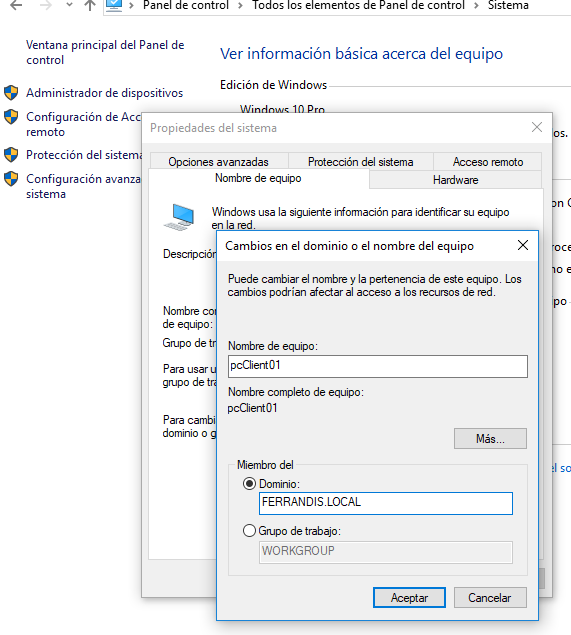
\includegraphics{png/18.png}

Vos demanarà un \textbf{compte amb drets d'Administrador en el Domini}.
Podem usar el que hem creat en la instal·lació del Server.

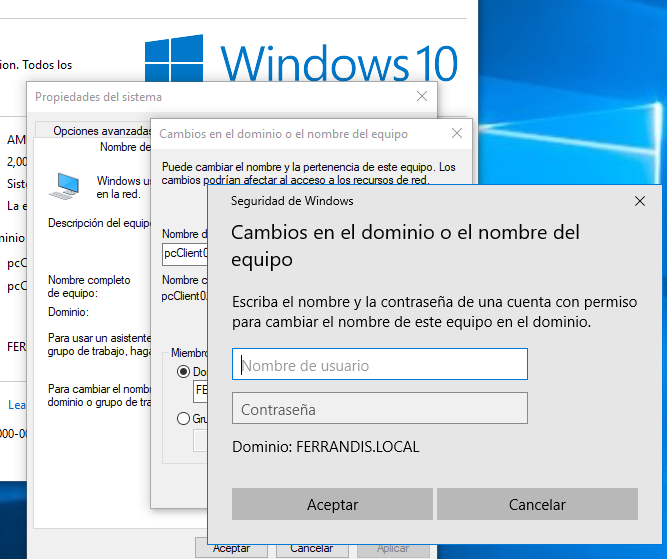
\includegraphics{png/demanacompteadministradordeldomini.png}

:computer: En el SERVIDOR, podeu visulitzar el PC afegit al Domini en
\textbf{Usuaris i Equips d'Active Directoy}

Podeu entrar executant el \textbf{dsa.msc} ( Winn + R \ldots)

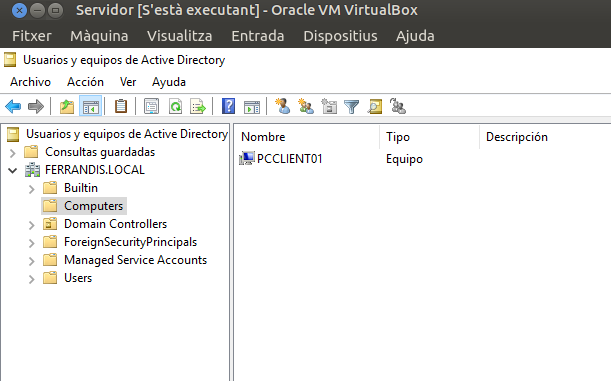
\includegraphics{png/20.png}

\subsection{3. Iniciem sessió al Domini des del
Client}\label{iniciem-sessiuxf3-al-domini-des-del-client}

Per iniciar sessión en el domini des del Windows 1X, encara que podríem
usar algun usuari de domini predefinit com el mateix compte
d'Administrador, el que farem prèviament és crear un usuari nou. De fet
el normal és disposar de comptes per als usuaris reals de l'organizació.

\textbf{3.1 Creem l'usuari}

Des de l'Administrador del Servidor veiem les dos funcionalitats des
d'on podem accedir a la gestió de comptes.

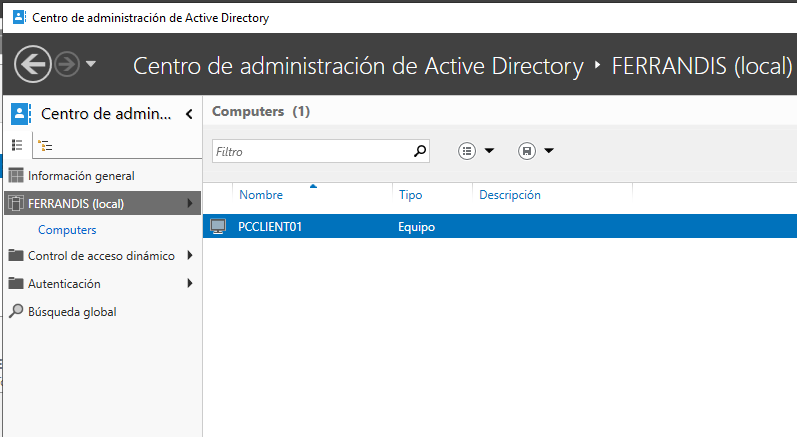
\includegraphics{png/centroadministracionactivedirectory.png}

Centro de Administración del Active Directory

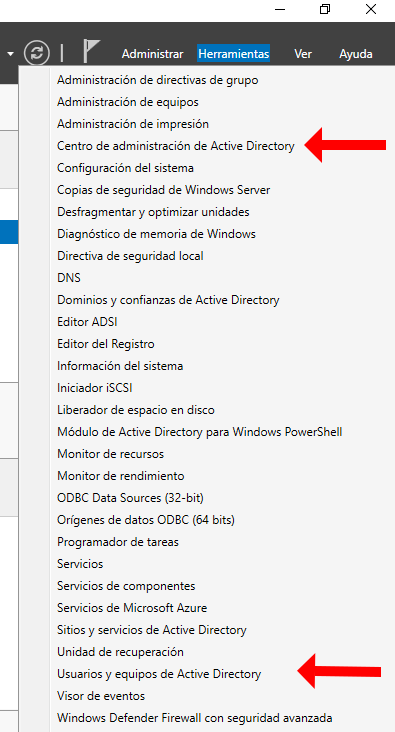
\includegraphics{png/administradordelservidorADDS.png}

Usuarios y equipos del AD

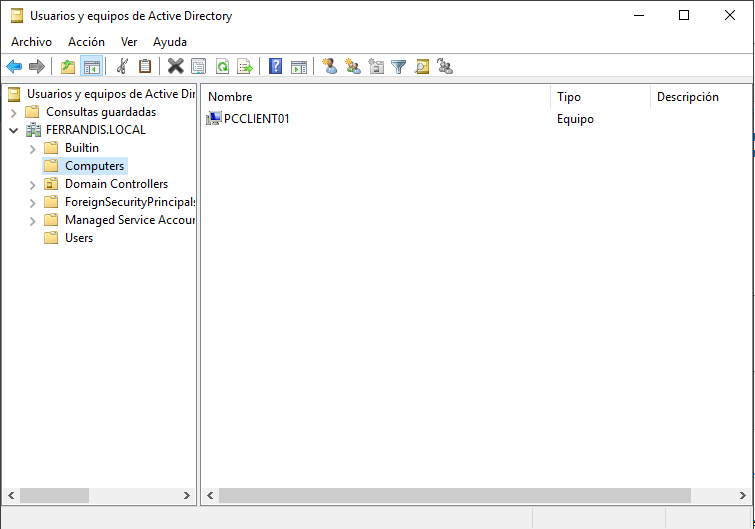
\includegraphics{png/usuariosyequiposactivedirectory.png}

\textbf{Contrasenya amb requisits de complexitat}

Si intentem indicar una contrasenay senzill, curta, fàcil\ldots{} vorem
que no ens ho permet el SO. Més avant tractarem estos requisits i altres
característiques de la contrassenya i dels comptes.

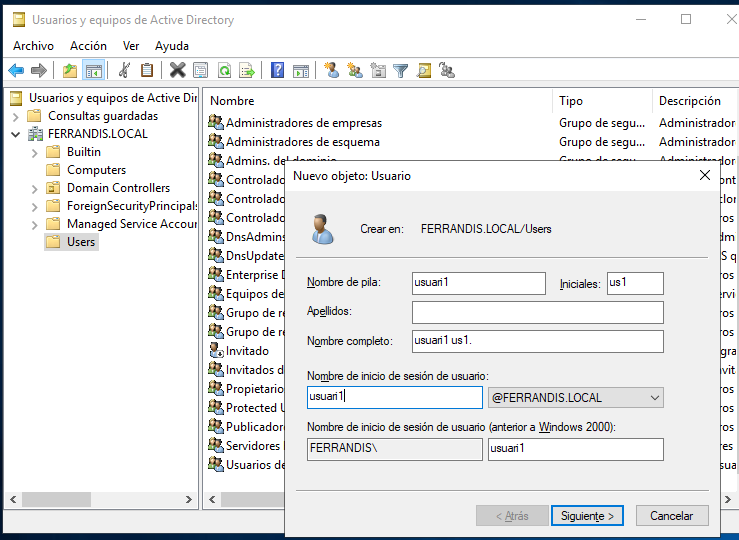
\includegraphics{png/creausuaridomini.png}

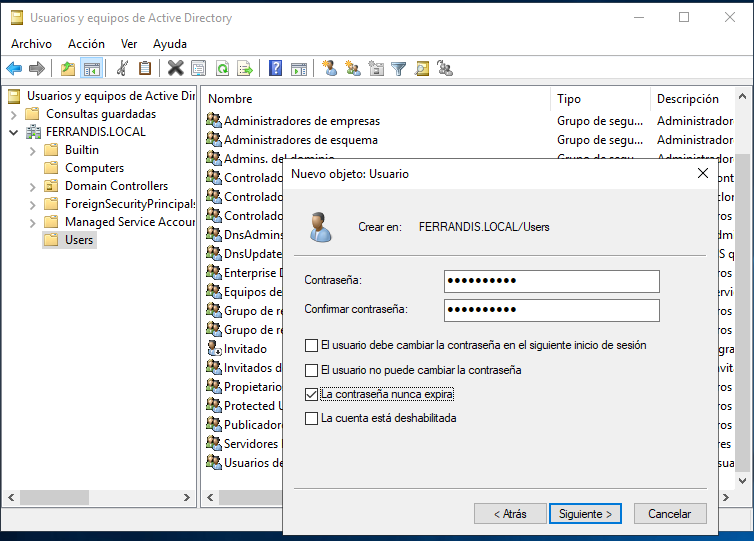
\includegraphics{png/creausuaridominicontrasenya.png}

\textbf{El grup ``Usuarios del dominio''}

Observem que tots els usuaris del domini perntanyen a un grup preexitent
``Usuarios del Dominio''.

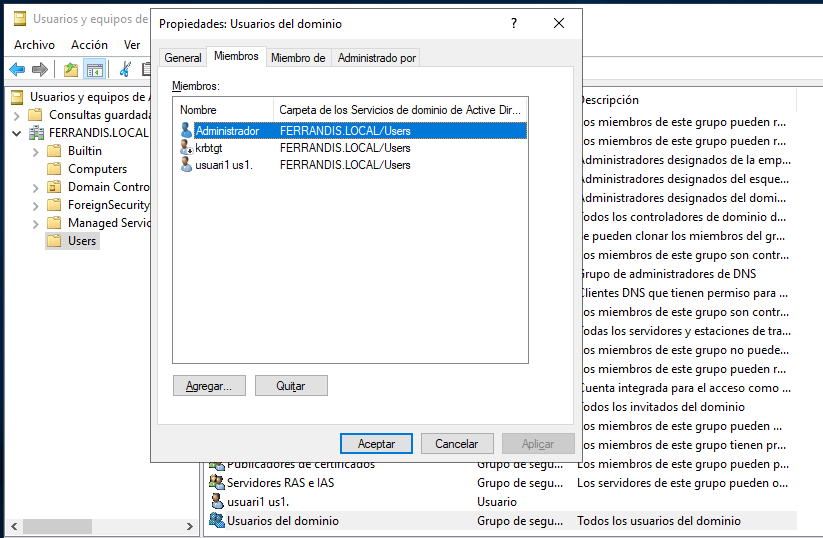
\includegraphics{png/grupousuariosdeldominio.png}

\textbf{Iniciem sessió}

Com la màquina client ja pertany al domini, en iniciar sessió del
Windows 1x només cal selecionar un usuari del domini nou usuari.

\begin{quote}
Nota

Més avant vorem amb un poc més de detall la configuració de les entitats
del AD i les seues relacions. També tenim documentació per a la seua
gestió mitjançant cmdLets i scripts fets amb Powershell
\end{quote}

\textbf{Característiques dels usuaris de domini al client}

\begin{itemize}
\item
  El nou usuari (usuari1) tindrà un perfil al PC Client però
\item
  NO és Administrador del PC Client. Qualsevol canvi de configuració que
  intente fer, el Windows 1x li demanarà les credencials d'Administrador
  local (``tomas'', a l'exemple)
\item
  Quan vullguen inicar sessió amb l'Administrador del Windows 1x, devem
  canviar de ``domini'', això ho farem avantposant al ``login'' el
  \textbf{nom de la màquina local} (a l'exemple:
  ``PCCLient\textbackslash tomas'' )
\item
  Amb este usuari, si es podria fer Administrador Local ( del Windows 1x
  ) a l'usuari del domini ( ``usuari1'')
\item
  Quan iniciem sessió en el domini, caldrà fixar-se i, si cal,
  avantposar també el \textbf{nom netbios del domini}
  (``FERRANDIS\textbackslash usuari1'')
\end{itemize}

\end{document}
